\subsection{ ক্ষেত্রফলের মান নির্ণয়ের পদ্ধতি }


 নির্দিষ্ট সমকালের সাহায্যে ক্ষেত্রফলের নির্ণয়ের জন্য নিচের ধাপ গুলি অনুসরণ করতে হবে। 

\begin{enumerate}
    \item প্রথমে প্রদত্ত আপেক্ষিক কে একটি খসড়া লেখচিত্র অঙ্কন করতে হবে।
    \item তারপর অফিস অভীষ্ট অঞ্চলটি চিত্রে নির্দেশিত করতে হবে।
    \item অবশেষে একটি নির্দিষ্ট সমাকলন গঠন করতে হবে এবং সমকালীন সীমা দুটি এরূপভাবে নির্বাচন করতে হবে যাতে স্বাধীন চলটি সমগ্র অঞ্চলে পরিবর্তিত হতে পারে ও সমকলটির মান নির্ণয় করতে হবে।

\end{enumerate}



\subsection{ $x = a,\: x = b,\: x$-অক্ষ এবং $y = f(x)$ বক্ররেখা দ্বারা সীমাবদ্ধ ক্ষেত্রে ক্ষেত্রফল}

\begin{minipage}{0.45\textwidth}
    \textbf{ক্ষেত্র-1:} যখন $f(x) > 0$ in $[a, b]$ :
    এক্ষেত্রে নির্ণয়ের ক্ষেত্রফল $= \int_{a}^{b} f(x)dx$

    
    \centering
    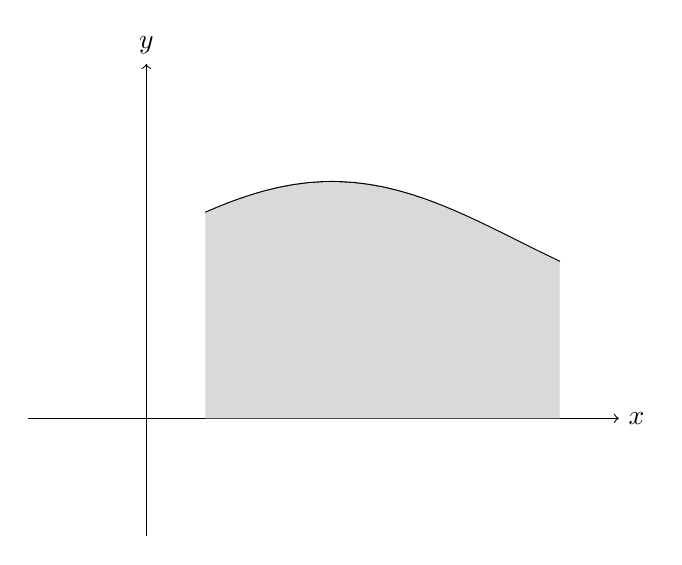
\begin{tikzpicture}[scale=1.5]
        %axis
        \draw[->] (-1,0) -- (4,0) node[right]{$x$};
        \draw[->] (0,-1) -- (0,3) node[above]{$y$};

        %function
        \draw[domain=0.5:3.5,smooth,variable=\x,thick] plot ({\x},{0.5*sin(\x r)+1.5});
        
        % Filling the area
        \fill[gray!30, domain=0.5:3.5, variable=\x]
        (0.5,0) -- plot ({\x},{0.5*sin(\x r)+1.5}) -- (3.5,0) -- cycle;

        
    \end{tikzpicture}

    \captionof{figure}{Graph of $\int_{0}^{2} x \, dx$}
    \label{fig:integral-graph}

    

\end{minipage}
\hfill
\begin{minipage}{0.45\textwidth}

    \textbf{ক্ষেত্র-2:} যখন $f(x) < 0$ in $[a,b]$ :
    এক্ষেত্রে নির্ণয়ের ক্ষেত্রফল $= \int_{a}^{b} (-f(x)) dx$

    \centering
    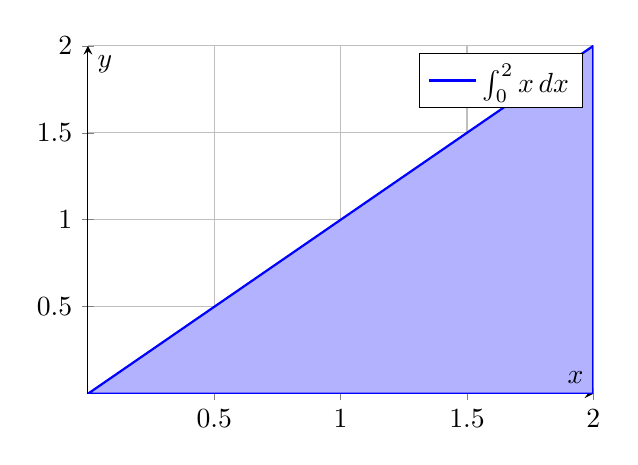
\begin{tikzpicture}
        \begin{axis}[
            domain=0:2,
            samples=100,
            axis lines=middle,
            xlabel=$x$,
            ylabel=$y$,
            grid=major,
            height=6cm,
            width=8cm,
            ]
            \addplot [blue, thick, fill=blue!30] {x} \closedcycle;
            \addlegendentry{$\int_{0}^{2} x \, dx$}
        \end{axis}
    \end{tikzpicture}
    \captionof{figure}{Graph of $\int_{0}^{2} x \, dx$}
    \label{fig:integral-graph2}
\end{minipage}

\newpage

\subsection{ $y = c,\: y = d,\: y$-অক্ষ এবং $x = f(y)$ বক্ররেখা দ্বারা সীমাবদ্ধ ক্ষেত্রে ক্ষেত্রফল}
\begin{minipage}{0.45\textwidth}
    
    \textbf{ক্ষেত্র-1:} যখন $f(y) > 0$ in $[c, d]$ :
    এক্ষেত্রে নির্ণয়ের ক্ষেত্রফল $= \int_{c}^{d} f(y)dy$

    
    \centering
    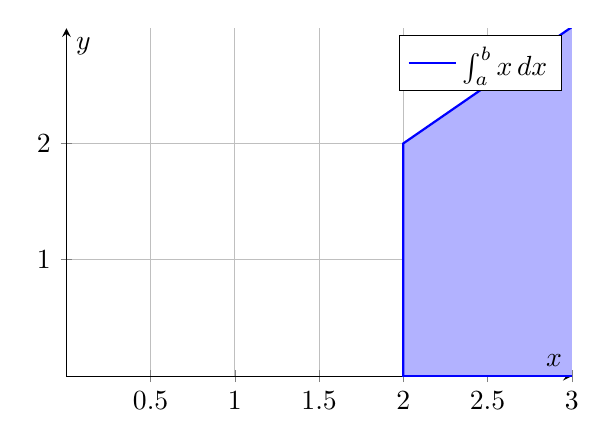
\begin{tikzpicture}
        \begin{axis}[
            domain=2:4,
            samples=100,
            axis lines=middle,
            xlabel=$x$,
            ylabel=$y$,
            grid=major,
            height=6cm,
            width=8cm,
            ymin=0,
            xmin = 0,
            xmax=3,
            ]
            \addplot [blue, thick, fill=blue!30] {x} \closedcycle;
            \addlegendentry{$\int_{a}^{b} x \, dx$}
        \end{axis}
    \end{tikzpicture}
    \captionof{figure}{Graph of $\int_{0}^{2} x \, dx$}
    \label{fig:integral-grapx}

    

\end{minipage}
\hfill
\begin{minipage}{0.45\textwidth}

    \textbf{ক্ষেত্র-2:} যখন $f(y) < 0$ in $[c,d]$ :
    এক্ষেত্রে নির্ণয়ের ক্ষেত্রফল $= \int_{c}^{d} (-f(y)) dx$

    \centering
    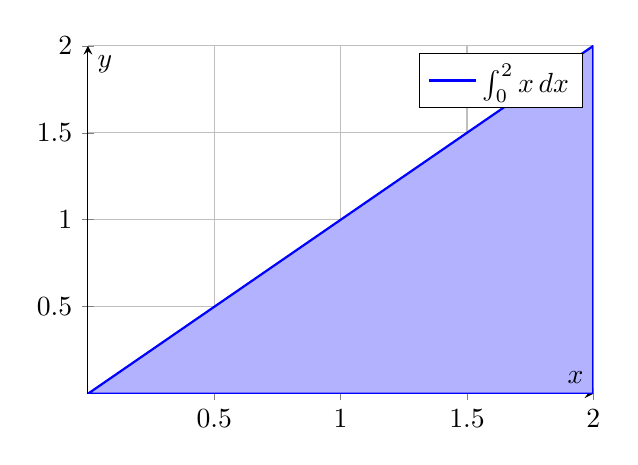
\begin{tikzpicture}
        \begin{axis}[
            domain=0:2,
            samples=100,
            axis lines=middle,
            xlabel=$x$,
            ylabel=$y$,
            grid=major,
            height=6cm,
            width=8cm,
            ]
            \addplot [blue, thick, fill=blue!30] {x} \closedcycle;
            \addlegendentry{$\int_{0}^{2} x \, dx$}
        \end{axis}
    \end{tikzpicture}
    \captionof{figure}{Graph of $\int_{0}^{2} x \, dx$}
    \label{fig:integral-grapd2}
\end{minipage}

\subsection{ $y = f_1(x),\: y = f_2(x),\:x=a$ এবং $x=b$ দ্বারা সীমাবদ্ধ ক্ষেত্রে ক্ষেত্রফল}

    \begin{minipage}{0.45\textwidth}
        চিত্র \ref{fig:intsegral-grapx}-এর ক্ষেত্রে

        নির্নিও খেত্রফল $=$ ABPQ ক্ষেত্রের ক্ষেত্রফল $=$ MNPQ ক্ষেত্রের ক্ষেত্রফল $-$ MNBA ক্ষেত্রের ক্ষেত্রফল

        $=\int_{a}^{b}f_1(x)dx - \int_{a}^{b}[f_1(x) - f_2(x)]dx = \int_{a}^{b} (y$ of upper curve $- y$ of lower curve$)dx$ 

        \centering
        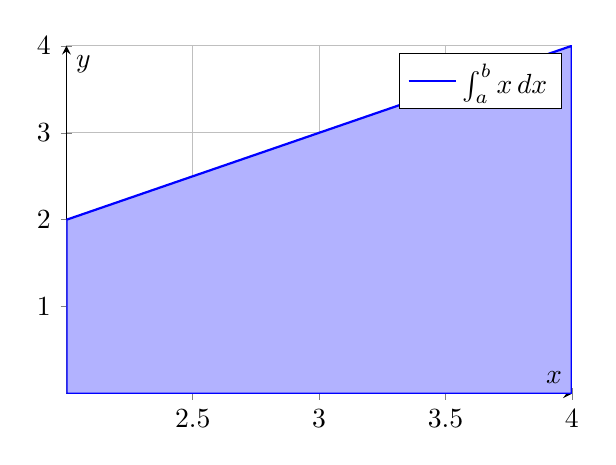
\begin{tikzpicture}
            \begin{axis}[
                domain=2:4,
                samples=100,
                axis lines=middle,
                xlabel=$x$,
                ylabel=$y$,
                grid=major,
                height=6cm,
                width=8cm,
                ymin=0,
                ]
                \addplot [blue, thick, fill=blue!30] {x} \closedcycle;
                \addlegendentry{$\int_{a}^{b} x \, dx$}
            \end{axis}
        \end{tikzpicture}
        \captionof{figure}{Graph of $\int_{0}^{2} x \, dx$}
        \label{fig:intsegral-grapx}

        

    \end{minipage}
    \hfill
    \begin{minipage}{0.45\textwidth}
        
        চিত্র \ref{fig:intsegral-grapx}-এর ক্ষেত্রে

        নির্নিও খেত্রফল $=$ ABPQ ক্ষেত্রের ক্ষেত্রফল $=$ MNPQ ক্ষেত্রের ক্ষেত্রফল $+$ MNBA ক্ষেত্রের ক্ষেত্রফল

        $=\int_{a}^{b}f_1(x)dx - \int_{a}^{b}(- f_2(x))dx$ $[\because f_2(x) < 0 ] = \int_{a}^{b}[f_1(x) - f_2(x)]dx$\\
        $= \int_{a}^{b} (y$ of upper curve $- y$ of lower curve$)dx$ 

        \centering
        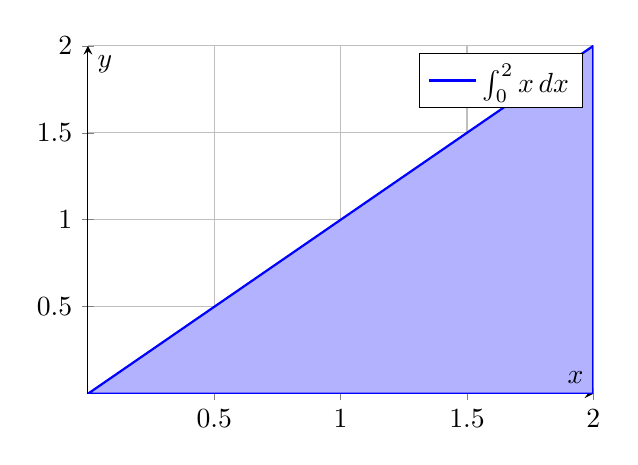
\begin{tikzpicture}
            \begin{axis}[
                domain=0:2,
                samples=100,
                axis lines=middle,
                xlabel=$x$,
                ylabel=$y$,
                grid=major,
                height=6cm,
                width=8cm,
                ]
                \addplot [blue, thick, fill=blue!30] {x} \closedcycle;
                \addlegendentry{$\int_{0}^{2} x \, dx$}
            \end{axis}
        \end{tikzpicture}
        \captionof{figure}{Graph of $\int_{0}^{2} x \, dx$}
        \label{fig:sintegral-grapd2}
    \end{minipage}

\subsection{ $x=f_1(y),\: x = f_2(y),\: y = c$ এবং $y = d$ দ্বারা সীমাবদ্ধ ক্ষেত্রে ক্ষেত্রফল}

\begin{minipage}{0.45\textwidth}
    
    পূর্বের ন্যায় এক্ষেত্রেও [\ref{fig:integral-grapd2} নং চিত্রের ক্ষেত্রে]

    নির্ণয় ক্ষেত্রফল $= \int_{c}^{d}f_1(y)dy - \int_{c}^{d}f_2(y)dy = \int_{c}^{d}[f_1(y) - f_2(y)]dy$
    $= \int_{c}^{d}[x$ of upper curve $-x$ of lower curve$]dy$

    \centering
    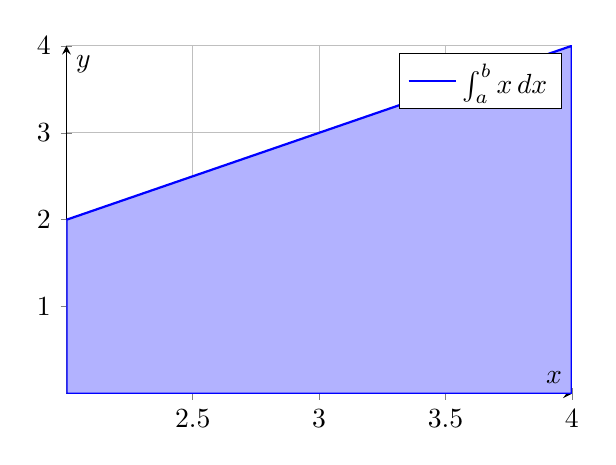
\begin{tikzpicture}
        \begin{axis}[
            domain=2:4,
            samples=100,
            axis lines=middle,
            xlabel=$x$,
            ylabel=$y$,
            grid=major,
            height=6cm,
            width=8cm,
            ymin=0,
            ]
            \addplot [blue, thick, fill=blue!30] {x} \closedcycle;
            \addlegendentry{$\int_{a}^{b} x \, dx$}
        \end{axis}
    \end{tikzpicture}
    \captionof{figure}{Graph of $\int_{0}^{2} x \, dx$}
    \label{fig:intsegral-grapx}

    

\end{minipage}
\hfill
\begin{minipage}{0.45\textwidth}

    পূর্বের ন্যায় এক্ষেত্রেও [\ref{fig:integral-grapd2} নং চিত্রের ক্ষেত্রে]

    নির্ণয় ক্ষেত্রফল $= \int_{c}^{d}f_1(y)dy + \int_{c}^{d}(-f_2(y))dy = \int_{c}^{d}[f_1(y) - f_2(y)]dy$
    $= \int_{c}^{d}[x$ of upper curve $-x$ of lower curve$]dy$

    \centering
    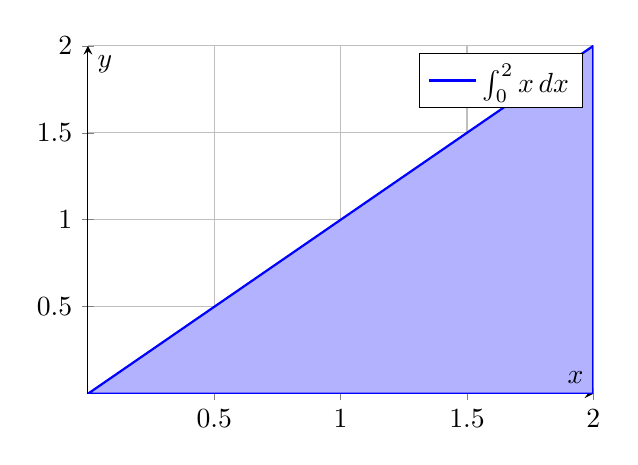
\begin{tikzpicture}
        \begin{axis}[
            domain=0:2,
            samples=100,
            axis lines=middle,
            xlabel=$x$,
            ylabel=$y$,
            grid=major,
            height=6cm,
            width=8cm,
            ]
            \addplot [blue, thick, fill=blue!30] {x} \closedcycle;
            \addlegendentry{$\int_{0}^{2} x \, dx$}
        \end{axis}
    \end{tikzpicture}
    \captionof{figure}{Graph of $\int_{0}^{2} x \, dx$}
    \label{fig:sintegral-grapd2}
\end{minipage}

\subsection{দুটি বক্ররেখার দ্বারা সীমাবদ্ধ ক্ষেত্রে ক্ষেত্রফল}
    চিত্র \ref{fig:integral-grapd2}-এর ক্ষেত্রে, $y = f_1(x)$ এবং $y = f_2(x)$ 
    বক্ররেখা দুটি পরস্পরকে $A$ এবং $B$ বিন্দুতে ছেদ করছে এবং ছেদবিন্দু দুটি ভুজ যথাক্রমে $a$ এবং $b$।
    এখন $x = a$ এবং $x = b$ সমান্তরাল রেখাদুটির মধ্যে সমস্ত আচ্ছাদিত অঞ্চলটি আছে।

    এরকম ক্ষেত্রে নির্ণয় ক্ষেত্রফল\\ $= \int_{a}^{b}[f_1(x) -f f_2(x)]dx = \int_{a}^{b}[y$ of upper curve $- y$ of lower curve$]dx$

    আবার যদি সমস্ত আচ্ছাদিত অঞ্চলটি $y = c$ এবং $y = d$ সমান্তরাল লেখা দুটির মধ্যে থাকে তবে নির্ণেয় ক্ষেত্রফলটিকে
    $\int_{c}^{d}[x$ of upper curve $- x$ of lower curve$]dy$-এর দাড়াও নির্ণয় করা যেতে পারে।

    \begin{figure}[h]
    \centering
    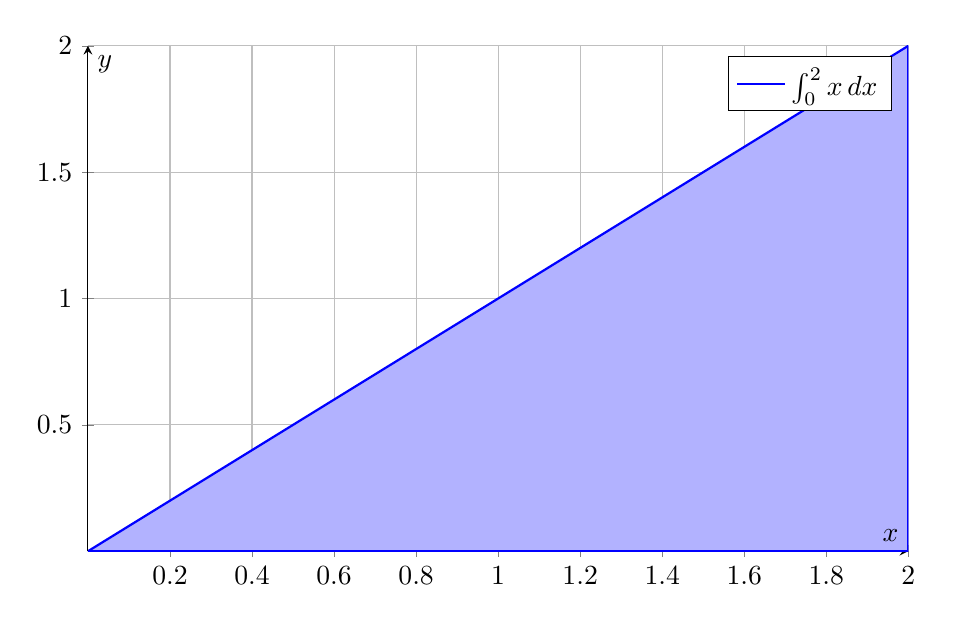
\begin{tikzpicture}
    \begin{axis}[
        domain=0:2,
        samples=100,
        axis lines=middle,
        xlabel=$x$,
        ylabel=$y$,
        grid=major,
        height=8cm,
        width=12cm,
        ]
        \addplot [blue, thick, fill=blue!30] {x} \closedcycle;
        \addlegendentry{$\int_{0}^{2} x \, dx$}
    \end{axis}
    \end{tikzpicture}
    \caption{Graph of $\int_{0}^{2} x \, dx$}
    \label{fig:integralsdfssd-graph}
    \end{figure}

\newpage
\subsection{যখন $y = f(x)$ বক্ররেখা $[a,b]$ অন্তরালের মধ্যে $x$-অক্ষকে ছেদ করে}

    ধরা যাক, $y = f(x)$ বড়ক্রটি $x$-অক্ষকে $x = c$ বিন্দুতে $(a < c < b)$ ছেদ করে [চিত্র-\ref{fig:integral-grapd2}]।
    এ ক্ষেত্রে $x$-অক্ষের উপরের অংশ জন্য $f(x) > 0$ কিন্তু $x$-অক্ষর নীচের অংশের জন্য $f(x) < 0$
    এক্ষেত্রে নির্ণয় ক্ষেত্রফল $= \int_{c}^{a}[-f(y)]dy + \int_{c}^{b}f(y)dy$

\subsection{যখন $x = f(y)$ বক্ররেখা $[c,d]$ অন্তরালের মধ্যে $y$-অক্ষকে ছেদ করে}

   
    এক্ষেত্রে নির্ণয় ক্ষেত্রফল $= \int_{c}^{a}f(y)dy + \int_{a}^{d}[-f(y)]dy$



\subsection{উদাহরণ}

\textbf{ উদাহরণ-1: }
$\frac{x}{2} + \frac{y}{3} = 1$ সরলরেখাটি অঙ্কদ্বয়ের সঙ্গে যে ত্রিভুজটি উৎপন্ন করে তার ক্ষেত্রফল নির্দিষ্ট সমকালের সাহায্যে নির্ণয়।

\textbf{ সমাধান: } $\frac{x}{2} + \frac{y}{3} = 1$ [ সরলরেখাটি অক্ষদ্বয়কে যথাক্রমে $(2,0)$ ও $(0,3)$ বিন্দুতে ছেদ করে।]

বা, $3x +  2y = 6$ বা, $y = \frac{x}{2} + \frac{y}{3} = 1$

$\therefore$ নির্ণেয় খেত্রফল
$$= \int_{0}^{2}dx = \int_{0}^{2} \frac{6-3x}{2}dx  = \int_{0}^{2}\left(3 - \frac{3}{2}x\right)dx$$

$ \left[3x - \frac{3}{4}x^2\right]_0^2 = (6-3) - ( 0 -0) = 3$ বার্গ একক।

\textbf{ উদাহরণ-2: }
$ x = 0, y -x  $ এবং $ 2y + x = 6$ সরলরেখা তিনটি দ্বারা সীমাবদ্ধ ক্ষেত্রের ক্ষেত্রফল নির্দিষ্ট সমকালের সাহায্যে নির্ণয় কর।

\textbf{ সমাধান: } $x = 0$ হলে $y$-অক্ষ। $y=x ...(1)$ বিন্দুগামী সরলরেখা যা $x$-অক্ষর ধনাত্মক দিকের সঙ্গে $45^{\circ}$ কোণ উঁত্পন্ন করে।

$2y + x = 6$ বা $\frac{x}{6} + \frac{y}{3} = 1 ...(2)$

এখন, (1) ও (2) সমাধান করে পাই, $3x = 6 $ বা, $x=2$

$\therefore y = 2$ 

$\therefore$ (1) ও (2)-এর ছেদবিন্দু A $(2,2)$ (2) নং সরলরেখাটি $y$-অক্ষকে B(0,3) বিন্দুতে ছেদ করে।

$\therefore$ নির্ণেয় খেত্রফল $= \int_{0}^{2}x dy$ on (1) $+ \int_{2}^{3}x dy$ on (2)

$=\int_{0}^{2}y dy + \int_{2}^{3}(6-2y)dy = \left[\frac{y^2}{2}\right]_0^2 + \left[6y - \frac{2y^2}{2}\right]_2^3$

$=2 + (18 - 9) - (12 - 4) = 2 + 9 - 8 = 3$ বর্গ একক।

\textbf{উদাহরণ-3:} সমাকলনের $x^2 + y^2 = a^2$ বৃত্তের ক্ষেত্রফল নির্ণয় করো।

\textbf{সমাধান:} $x^2+y^2= a^2$ বা $y = \root{a^2 - x^2}$ (প্রথম পাদে)

$\therefore$ নির্ণের ক্ষেত্রফল $= 4 \int_{0}^{a} y dx$ [প্রথম পাদের ক্ষেত্রফলকে এ দিয়ে গুণ করা হয়েছে ।]

$$= 4\int_{0}^{a}\root{a^2 - x^2}dx = 4\left[ \frac{x\root{a^2 - x^2}}{2} + \frac{a^2}{2}\sin^-1\frac{x}{a} \right]_0^a$$
$$= \left[0 + \frac{a^2}{2}\arcsin\frac{a}{a}-0-0\right] =  2a^2 \arcsin1$$
$= 2a^2 \frac{\pi}{2} = \pi a^2$ বর্গ একক।


% ) উদাহরণ-4 16s অধিবৃত্ত এবং এর নাভিলম্ব দ্বারা সীমাবদ্ধ ক্ষেত্রের ক্ষেত্রফল সমাকলনের সাহায্যে নির্ণয় করো।

% # সমधानy 16r বা y = 4√ (প্রথম পাদে।

% নাভি S এর স্থান (40)

% :. নির্ণেয় ক্ষেত্রফল = 2 10y dx 1 এখানে প্রথম পাদের ক্ষেত্রফলকে 2 দিয়ে গুণ করা হয়েছে।।

% (S(40)

% = 2][4√= dx = 8

% 128 3 বর্গ একক।





\newpage


